% gen_server Complete Tutorial
% Compile with: xelatex gen_server_tutorial.tex (run twice for TOC)
\documentclass[a4paper,11pt]{article}

% ============================================================
% Packages
% ============================================================
\usepackage{fontspec}
\usepackage{xeCJK}
\setCJKmainfont[BoldFont=STHeiti, ItalicFont=STKaiti]{STSong}
\setCJKsansfont{STHeiti}
\setCJKmonofont{STFangsong}

\usepackage[margin=2.5cm]{geometry}
\usepackage{graphicx}
\usepackage{xcolor}
\usepackage{hyperref}
\usepackage{listings}
\usepackage{booktabs}
\usepackage{longtable}
\usepackage{enumitem}
\usepackage{tikz}
\usepackage{tcolorbox}
\usepackage{fancyhdr}
\usepackage{titlesec}
\usepackage{amsmath}
\usepackage{amssymb}
\usepackage{float}

\usetikzlibrary{arrows.meta, positioning, shapes.geometric, fit, calc, backgrounds, decorations.pathreplacing}

\tcbuselibrary{listings, skins, breakable}

% ============================================================
% Color Definitions
% ============================================================
\definecolor{erlred}{HTML}{A4070A}
\definecolor{erlblue}{HTML}{2B5EA7}
\definecolor{erlgreen}{HTML}{2E7D32}
\definecolor{erlyellow}{HTML}{F9A825}
\definecolor{erlpurple}{HTML}{6A1B9A}
\definecolor{codebg}{HTML}{F5F5F5}
\definecolor{codeborder}{HTML}{CCCCCC}
\definecolor{tipbg}{HTML}{E8F5E9}
\definecolor{warnbg}{HTML}{FFF3E0}
\definecolor{notebg}{HTML}{E3F2FD}
\definecolor{darkgray}{HTML}{333333}
\definecolor{lightgray}{HTML}{EEEEEE}

% ============================================================
% Hyperref Setup
% ============================================================
\hypersetup{
    colorlinks=true,
    linkcolor=erlblue,
    urlcolor=erlpurple,
    citecolor=erlgreen,
    pdftitle={gen\_server Complete Tutorial},
    pdfauthor={Erlang OTP Tutorial},
    bookmarksnumbered=true,
}

% ============================================================
% Code Listing Style
% ============================================================
\lstdefinelanguage{erlang}{
    morekeywords={module, export, import, behaviour, behavior, spec, type,
        record, define, include, ifdef, ifndef, else, endif, undef,
        case, of, end, if, receive, after, when, fun, try, catch, throw,
        begin, spawn, spawn_link, register, self, send, ok, error,
        true, false, undefined, infinity, timeout, noreply, reply, stop,
        hibernate, ignore, normal, process_flag, trap_exit, monitor_node},
    sensitive=true,
    morecomment=[l]{\%},
    morestring=[b]",
    morestring=[b]',
}

\lstdefinestyle{erlangstyle}{
    language=erlang,
    basicstyle=\ttfamily\small,
    keywordstyle=\color{erlblue}\bfseries,
    commentstyle=\color{erlgreen}\itshape,
    stringstyle=\color{erlred},
    numberstyle=\tiny\color{gray},
    numbers=left,
    numbersep=8pt,
    backgroundcolor=\color{codebg},
    frame=single,
    rulecolor=\color{codeborder},
    breaklines=true,
    breakatwhitespace=true,
    tabsize=4,
    showstringspaces=false,
    captionpos=b,
    xleftmargin=1.5em,
    framexleftmargin=1em,
    aboveskip=1em,
    belowskip=0.8em,
}

\lstdefinestyle{shellstyle}{
    basicstyle=\ttfamily\small,
    backgroundcolor=\color{darkgray},
    rulecolor=\color{darkgray},
    frame=single,
    breaklines=true,
    showstringspaces=false,
    keywordstyle=\color{white},
    commentstyle=\color{white},
    stringstyle=\color{white},
    basicstyle=\ttfamily\small\color{white},
    xleftmargin=1.5em,
    framexleftmargin=1em,
    aboveskip=1em,
    belowskip=0.8em,
}

\lstset{style=erlangstyle}

% ============================================================
% Custom tcolorbox Environments
% ============================================================
\newtcolorbox{tipbox}[1][]{
    colback=tipbg, colframe=erlgreen!80!black,
    fonttitle=\bfseries, title={#1},
    arc=2mm, boxrule=0.8pt,
    left=6pt, right=6pt, top=4pt, bottom=4pt,
    breakable,
}

\newtcolorbox{warnbox}[1][]{
    colback=warnbg, colframe=erlyellow!80!black,
    fonttitle=\bfseries, title={#1},
    arc=2mm, boxrule=0.8pt,
    left=6pt, right=6pt, top=4pt, bottom=4pt,
    breakable,
}

\newtcolorbox{notebox}[1][]{
    colback=notebg, colframe=erlblue!80!black,
    fonttitle=\bfseries, title={#1},
    arc=2mm, boxrule=0.8pt,
    left=6pt, right=6pt, top=4pt, bottom=4pt,
    breakable,
}

% ============================================================
% Header / Footer
% ============================================================
\pagestyle{fancy}
\fancyhf{}
\fancyhead[L]{\small\textit{gen\_server Complete Tutorial}}
\fancyhead[R]{\small\textit{Erlang/OTP}}
\fancyfoot[C]{\thepage}
\renewcommand{\headrulewidth}{0.4pt}

% ============================================================
% Title Formatting
% ============================================================
\titleformat{\section}
    {\LARGE\bfseries\color{erlblue}}
    {\thesection}{1em}{}[\vspace{-0.5em}\rule{\textwidth}{0.8pt}]

\titleformat{\subsection}
    {\Large\bfseries\color{erlblue!80!black}}
    {\thesubsection}{0.8em}{}

\titleformat{\subsubsection}
    {\large\bfseries\color{erlblue!60!black}}
    {\thesubsubsection}{0.6em}{}

% ============================================================
% Document Begin
% ============================================================
\begin{document}

% ---- Title Page ----
\begin{titlepage}
\centering
\vspace*{2cm}

\begin{tikzpicture}
    % Erlang logo-inspired decoration
    \foreach \i in {0,1,...,5} {
        \draw[erlblue!50, line width=1.5pt, opacity=0.3+\i*0.1]
            (0+\i*0.3, 0) .. controls (2+\i*0.2, 1.5-\i*0.2) and (4-\i*0.2, -1+\i*0.15) .. (6, 0.5-\i*0.1);
    }
    \node[font=\fontsize{48}{52}\selectfont\bfseries, text=erlblue] at (3, -1.5) {gen\_server};
    \node[font=\fontsize{24}{28}\selectfont, text=erlblue!70!black] at (3, -3) {完全教程};
\end{tikzpicture}

\vspace{2cm}

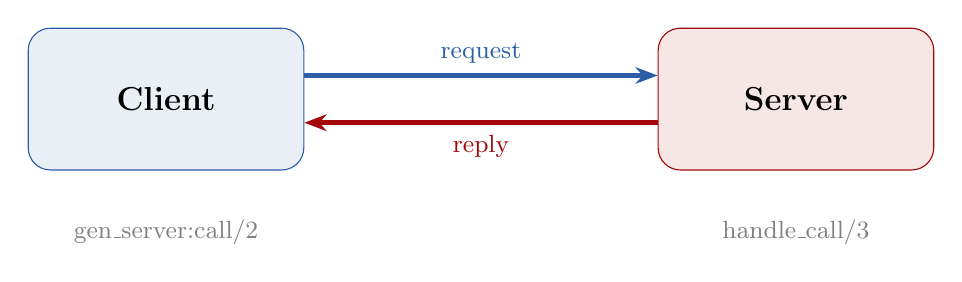
\begin{tikzpicture}
    % Client-Server illustration
    \node[draw=erlblue, fill=erlblue!10, rounded corners=8pt, minimum width=3.5cm, minimum height=1.8cm, font=\large\bfseries] (client) at (0,0) {Client};
    \node[draw=erlred, fill=erlred!10, rounded corners=8pt, minimum width=3.5cm, minimum height=1.8cm, font=\large\bfseries] (server) at (8,0) {Server};

    \draw[-{Stealth[length=8pt]}, line width=2pt, erlblue]
        ([yshift=3mm]client.east) -- node[above, font=\small] {request} ([yshift=3mm]server.west);
    \draw[-{Stealth[length=8pt]}, line width=2pt, erlred]
        ([yshift=-3mm]server.west) -- node[below, font=\small] {reply} ([yshift=-3mm]client.east);

    \node[below=5mm of client, font=\small\color{gray}] {gen\_server:call/2};
    \node[below=5mm of server, font=\small\color{gray}] {handle\_call/3};
\end{tikzpicture}

\vspace{3cm}

{\large\color{darkgray} From Raw Processes to OTP Behaviors}

\vspace{1cm}

{\normalsize\color{gray} Erlang/OTP $\cdot$ Behavior Pattern $\cdot$ Concurrent Programming}

\vfill
{\small\today}
\end{titlepage}

% ---- Table of Contents ----
\newpage
\tableofcontents
\newpage

% ============================================================
% Section 1: Overview
% ============================================================
\section{概述}

\subsection{什么是 gen\_server？}

\texttt{gen\_server} 是 OTP 框架中最核心的行为模式（behavior）之一。它将 Erlang 中常见的客户端--服务器（Client-Server）模式抽象为一个通用的库模块，开发者只需实现回调函数即可获得一个健壮的并发服务器。

\subsection{为什么需要 gen\_server？}

在 Erlang 中，许多不同的进程虽然解决的是不同的问题，但却遵循着相似的设计模式：

\begin{figure}[H]
\centering
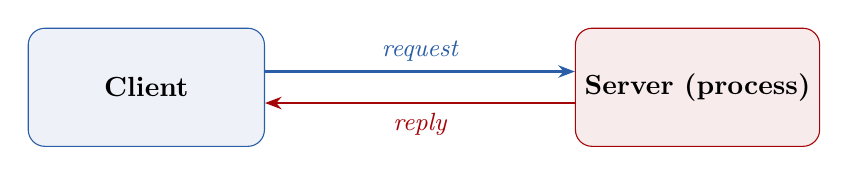
\begin{tikzpicture}
    \node[draw=erlblue, fill=erlblue!8, rounded corners=6pt,
          minimum width=3cm, minimum height=1.5cm, font=\bfseries] (c) at (0,0) {Client};
    \node[draw=erlred, fill=erlred!8, rounded corners=6pt,
          minimum width=3cm, minimum height=1.5cm, font=\bfseries] (s) at (7,0) {Server (process)};

    \draw[-{Stealth[length=6pt]}, thick, erlblue]
        ([yshift=2mm]c.east) -- node[above, font=\small\itshape] {request} ([yshift=2mm]s.west);
    \draw[-{Stealth[length=6pt]}, thick, erlred]
        ([yshift=-2mm]s.west) -- node[below, font=\small\itshape] {reply} ([yshift=-2mm]c.east);
\end{tikzpicture}
\caption{Client-Server 基本通信模式}
\label{fig:client-server-basic}
\end{figure}

这些模式包括：
\begin{itemize}[leftmargin=2em]
    \item 启动和初始化服务器进程
    \item 发送同步/异步请求
    \item 维护进程状态
    \item 处理错误和终止
    \item 热代码升级
\end{itemize}

OTP 将这些通用部分提取出来，封装为 \texttt{gen\_server} 行为模式库。

\subsection{架构图}

\begin{figure}[H]
\centering
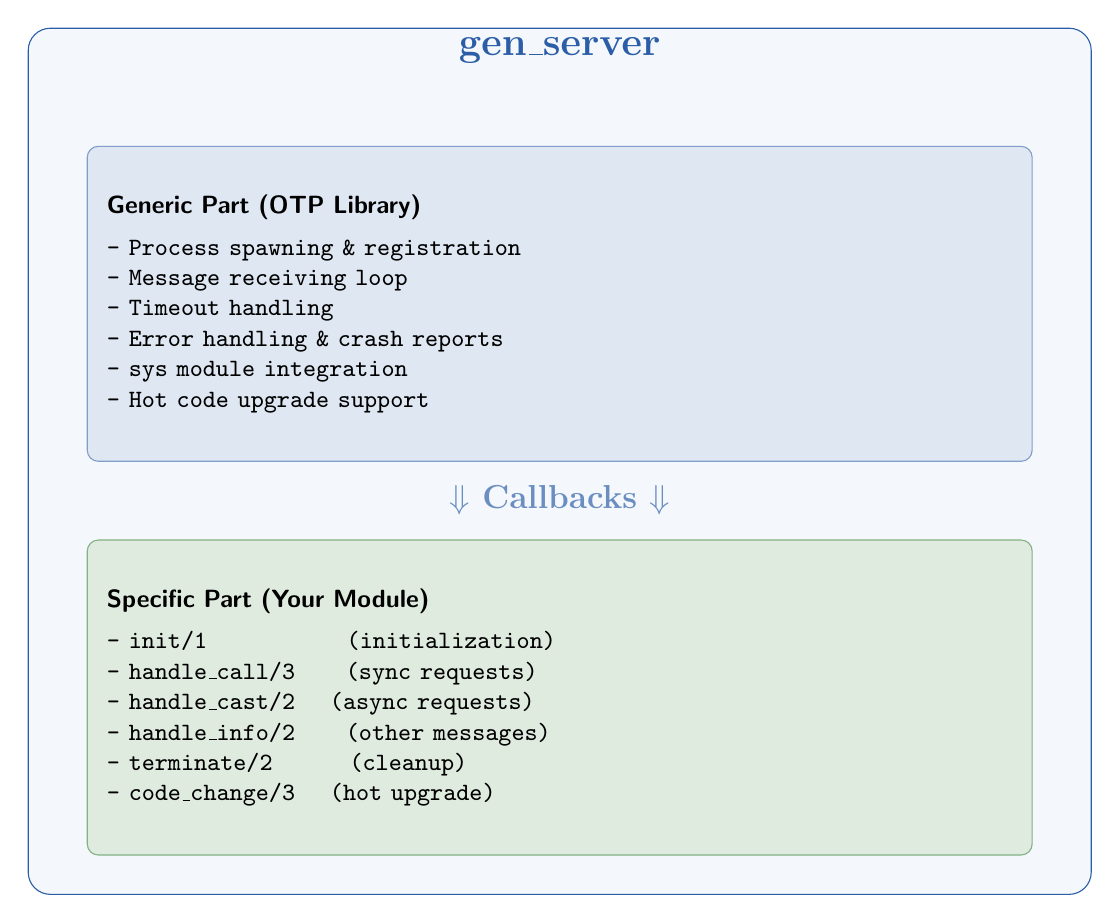
\begin{tikzpicture}[
    block/.style={draw, rounded corners=4pt, minimum width=12cm, text width=11.5cm, align=left, font=\small\ttfamily},
]
    % Outer frame
    \node[draw=erlblue, fill=erlblue!5, rounded corners=8pt,
          minimum width=13.5cm, minimum height=11cm] (outer) at (0,0) {};
    \node[font=\Large\bfseries\color{erlblue}, anchor=north] at (outer.north) {gen\_server};

    % Generic Part
    \node[block, fill=erlblue!15, draw=erlblue!60,
          minimum height=4cm] (generic) at (0, 2) {
        \textbf{\textsf{Generic Part (OTP Library)}} \\[4pt]
        - Process spawning \& registration \\
        - Message receiving loop \\
        - Timeout handling \\
        - Error handling \& crash reports \\
        - sys module integration \\
        - Hot code upgrade support
    };

    % Arrow
    \node[font=\large\bfseries\color{erlblue!70}] at (0, -0.5) {$\Downarrow$ Callbacks $\Downarrow$};

    % Specific Part
    \node[block, fill=erlgreen!15, draw=erlgreen!60,
          minimum height=4cm] (specific) at (0, -3) {
        \textbf{\textsf{Specific Part (Your Module)}} \\[4pt]
        - init/1 \quad\quad\quad\quad\quad (initialization) \\
        - handle\_call/3 \quad\; (sync requests) \\
        - handle\_cast/2 \quad (async requests) \\
        - handle\_info/2 \quad\; (other messages) \\
        - terminate/2 \quad\quad\; (cleanup) \\
        - code\_change/3 \quad (hot upgrade)
    };
\end{tikzpicture}
\caption{gen\_server 架构：通用部分与专用部分}
\label{fig:architecture}
\end{figure}


% ============================================================
% Section 2: Raw Erlang Process
% ============================================================
\section{从零开始：纯 Erlang 进程实现 Client-Server}

\begin{notebox}[源码文件]
\texttt{src/frequency\_raw.erl}
\end{notebox}

在使用 gen\_server 之前，我们先用纯 Erlang 进程实现一个频率分配服务器，理解底层原理。

\subsection{问题描述}

模拟一个移动通信基站的频率分配器：
\begin{itemize}[leftmargin=2em]
    \item 有一组可用频率 \texttt{[10, 11, 12, 13, 14, 15]}
    \item 客户端可以申请（allocate）一个频率
    \item 使用完毕后归还（deallocate）频率
\end{itemize}

\begin{figure}[H]
\centering
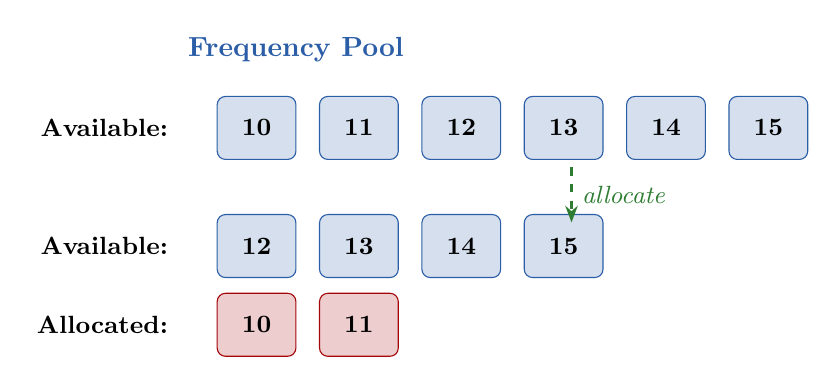
\begin{tikzpicture}[
    freq/.style={draw=erlblue, fill=erlblue!20, rounded corners=3pt,
                 minimum width=1cm, minimum height=0.8cm, font=\small\bfseries},
    used/.style={draw=erlred, fill=erlred!20, rounded corners=3pt,
                 minimum width=1cm, minimum height=0.8cm, font=\small\bfseries},
]
    % Title
    \node[font=\bfseries\color{erlblue}] at (0, 2) {Frequency Pool};

    % Available frequencies
    \node[font=\small\bfseries, anchor=east] at (-1.5, 1) {Available:};
    \foreach \f [count=\i from 0] in {10,11,12,13,14,15} {
        \node[freq] at (-0.5+\i*1.3, 1) {\f};
    }

    % After allocation
    \node[font=\small\bfseries, anchor=east] at (-1.5, -0.5) {Available:};
    \foreach \f [count=\i from 0] in {12,13,14,15} {
        \node[freq] at (-0.5+\i*1.3, -0.5) {\f};
    }
    \node[font=\small\bfseries, anchor=east] at (-1.5, -1.5) {Allocated:};
    \foreach \f [count=\i from 0] in {10,11} {
        \node[used] at (-0.5+\i*1.3, -1.5) {\f};
    }

    % Arrow
    \draw[-{Stealth[length=6pt]}, thick, erlgreen, dashed]
        (3.5, 0.5) -- node[right, font=\small\itshape] {allocate} (3.5, -0.2);
\end{tikzpicture}
\caption{频率分配器状态变化示意}
\label{fig:freq-pool}
\end{figure}

\subsection{代码结构}

\begin{lstlisting}[style=erlangstyle, caption={frequency\_raw.erl --- 纯 Erlang 进程实现}]
-module(frequency_raw).
-export([start/0, stop/0, allocate/0, deallocate/1]).
-export([init/0, demo/0]).

%% Start: spawn a process and register it
start() ->
    register(frequency_raw, spawn(frequency_raw, init, [])).

%% Client sends request and waits for reply
call(Message) ->
    frequency_raw ! {request, self(), Message},
    receive
        {reply, Reply} -> Reply
    end.

%% Server main loop
loop(Frequencies) ->
    receive
        {request, Pid, allocate} ->
            {NewFrequencies, Reply} = allocate(Frequencies, Pid),
            reply(Pid, Reply),
            loop(NewFrequencies);
        {request, Pid, {deallocate, Freq}} ->
            NewFrequencies = deallocate(Frequencies, Freq),
            reply(Pid, ok),
            loop(NewFrequencies);
        {request, Pid, stop} ->
            reply(Pid, ok)
    end.
\end{lstlisting}

\subsection{运行演示}

\begin{lstlisting}[style=shellstyle, caption={运行纯 Erlang 版本}]
$ cd src && make run_raw
Allocated frequency: 10
Allocated frequency: 11
Deallocated frequency: 10
Re-allocated frequency: 10
Server stopped.
\end{lstlisting}

\subsection{问题分析}

这个实现虽然能工作，但存在以下问题：

\begin{table}[H]
\centering
\begin{tabular}{@{}ll@{}}
\toprule
\textbf{问题} & \textbf{说明} \\
\midrule
代码耦合 & 通用的消息收发逻辑和业务逻辑混在一起 \\
无错误处理 & 服务器崩溃时客户端会永远阻塞 \\
无超时机制 & 没有请求超时保护 \\
不可重用 & 每个服务器都要重写消息循环 \\
无调试支持 & 没有 sys 模块集成 \\
\bottomrule
\end{tabular}
\caption{纯 Erlang 实现的问题}
\label{tab:raw-problems}
\end{table}


% ============================================================
% Section 3: Custom Generic Server
% ============================================================
\section{抽象通用模式：自定义 Generic Server}

\begin{notebox}[源码文件]
\texttt{src/my\_server.erl} + \texttt{src/frequency\_generic.erl}
\end{notebox}

\subsection{分离通用与专用代码}

将代码分为两部分：

\begin{figure}[H]
\centering
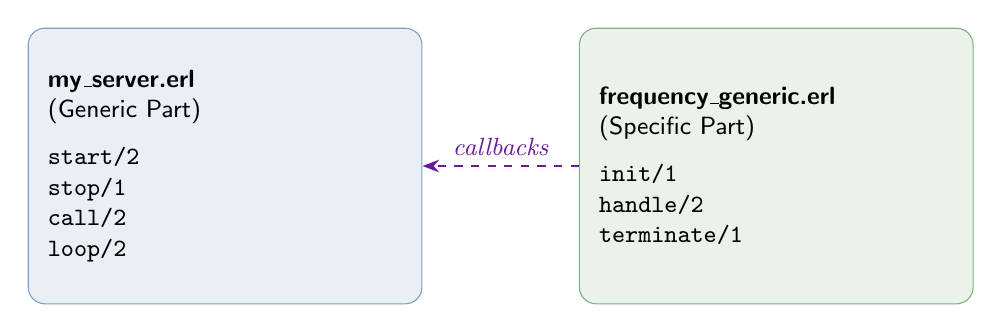
\begin{tikzpicture}[
    mod/.style={draw, rounded corners=6pt, minimum width=5cm, minimum height=3.5cm,
                text width=4.5cm, align=left, font=\small\ttfamily},
]
    \node[mod, fill=erlblue!10, draw=erlblue!60] (generic) at (0,0) {
        \textbf{\textsf{my\_server.erl}} \\
        \textsf{(Generic Part)} \\[6pt]
        start/2 \\
        stop/1 \\
        call/2 \\
        loop/2
    };

    \node[mod, fill=erlgreen!10, draw=erlgreen!60] (specific) at (7,0) {
        \textbf{\textsf{frequency\_generic.erl}} \\
        \textsf{(Specific Part)} \\[6pt]
        init/1 \\
        handle/2 \\
        terminate/1
    };

    \draw[-{Stealth[length=6pt]}, thick, erlpurple, dashed]
        (specific.west) -- node[above, font=\small\itshape] {callbacks} (generic.east);
\end{tikzpicture}
\caption{通用与专用代码分离}
\label{fig:separation}
\end{figure}

\subsection{通用服务器模块 (my\_server.erl)}

\begin{lstlisting}[style=erlangstyle, caption={my\_server.erl --- 自定义通用服务器}]
-module(my_server).
-export([start/2, stop/1, call/2]).

start(Name, Mod) ->
    register(Name, spawn(my_server, init, [Name, Mod])).

call(Name, Msg) ->
    Name ! {request, self(), Msg},
    receive {reply, Reply} -> Reply end.

%% Generic loop - dispatches to callback module
loop(Mod, State) ->
    receive
        {request, From, Msg} ->
            {NewState, Reply} = Mod:handle(Msg, State),
            reply(From, Reply),
            loop(Mod, NewState);
        {stop, From} ->
            Reply = Mod:terminate(State),
            reply(From, Reply)
    end.
\end{lstlisting}

\subsection{专用回调模块 (frequency\_generic.erl)}

\begin{lstlisting}[style=erlangstyle, caption={frequency\_generic.erl --- 回调模块}]
-module(frequency_generic).

%% Callback: initialize state
init(_Args) ->
    {get_frequencies(), []}.

%% Callback: handle requests
handle({allocate, Pid}, Frequencies) ->
    allocate(Frequencies, Pid);
handle({deallocate, Freq}, Frequencies) ->
    {deallocate(Frequencies, Freq), ok}.

%% Callback: cleanup
terminate(Frequencies) ->
    io:format("Terminating. State: ~p~n", [Frequencies]),
    ok.
\end{lstlisting}

\subsection{这就是 OTP 行为模式的本质！}

\begin{tipbox}[核心理解]
\textbf{理解了这个分离过程，就理解了 Erlang 的行为模式。}

本质上就是把代码分为通用的和专用的两部分，然后把通用的部分打包为可重用的库。

\hfill --- 《Erlang and OTP in Action》
\end{tipbox}


% ============================================================
% Section 4: OTP gen_server
% ============================================================
\section{OTP gen\_server 行为模式}

\begin{notebox}[源码文件]
\texttt{src/frequency\_otp.erl}
\end{notebox}

\subsection{从自定义到 OTP}

OTP 的 \texttt{gen\_server} 就是我们 \texttt{my\_server} 的工业级版本，额外提供了：

\begin{table}[H]
\centering
\begin{tabular}{@{}lccc@{}}
\toprule
\textbf{特性} & \textbf{my\_server} & \textbf{gen\_server} \\
\midrule
同步调用 (call)    & $\checkmark$ & $\checkmark$ \\
异步调用 (cast)    & ---        & $\checkmark$ \\
超时机制           & ---        & $\checkmark$ \\
错误处理           & ---        & $\checkmark$ \\
sys 模块集成       & ---        & $\checkmark$ \\
热代码升级         & ---        & $\checkmark$ \\
进程链接           & ---        & $\checkmark$ \\
format\_status     & ---        & $\checkmark$ \\
\bottomrule
\end{tabular}
\caption{my\_server vs gen\_server 功能对比}
\label{tab:comparison}
\end{table}

\subsection{声明行为模式}

\begin{lstlisting}[style=erlangstyle]
-module(frequency_otp).
-behaviour(gen_server).  %% Declare gen_server behavior
\end{lstlisting}

\subsection{启动服务器}

\begin{lstlisting}[style=erlangstyle, caption={启动 gen\_server}]
%% start_link: start and link to calling process
start_link() ->
    gen_server:start_link({local, frequency_otp}, ?MODULE, [], []).
%%                        ^^^^^^^^^^^^^^^^^^^    ^^^^^^  ^^  ^^
%%                        Registration           Module  Args Options
\end{lstlisting}

启动函数对比：

\begin{table}[H]
\centering
\begin{tabular}{@{}lcc@{}}
\toprule
\textbf{函数} & \textbf{链接} & \textbf{用途} \\
\midrule
\texttt{start\_link/3,4} & $\checkmark$ & 生产环境，配合 supervisor \\
\texttt{start/3,4}       & ---        & 开发测试，独立运行 \\
\bottomrule
\end{tabular}
\end{table}

\subsection{客户端 API}

\begin{lstlisting}[style=erlangstyle, caption={客户端 API --- call 与 cast}]
%% Synchronous call - waits for server reply
allocate() ->
    gen_server:call(frequency_otp, {allocate, self()}).

%% Asynchronous cast - returns immediately
deallocate(Frequency) ->
    gen_server:cast(frequency_otp, {deallocate, Frequency}).

%% Async stop
stop() ->
    gen_server:cast(frequency_otp, stop).
\end{lstlisting}

\subsection{消息流转图}

\begin{figure}[H]
\centering
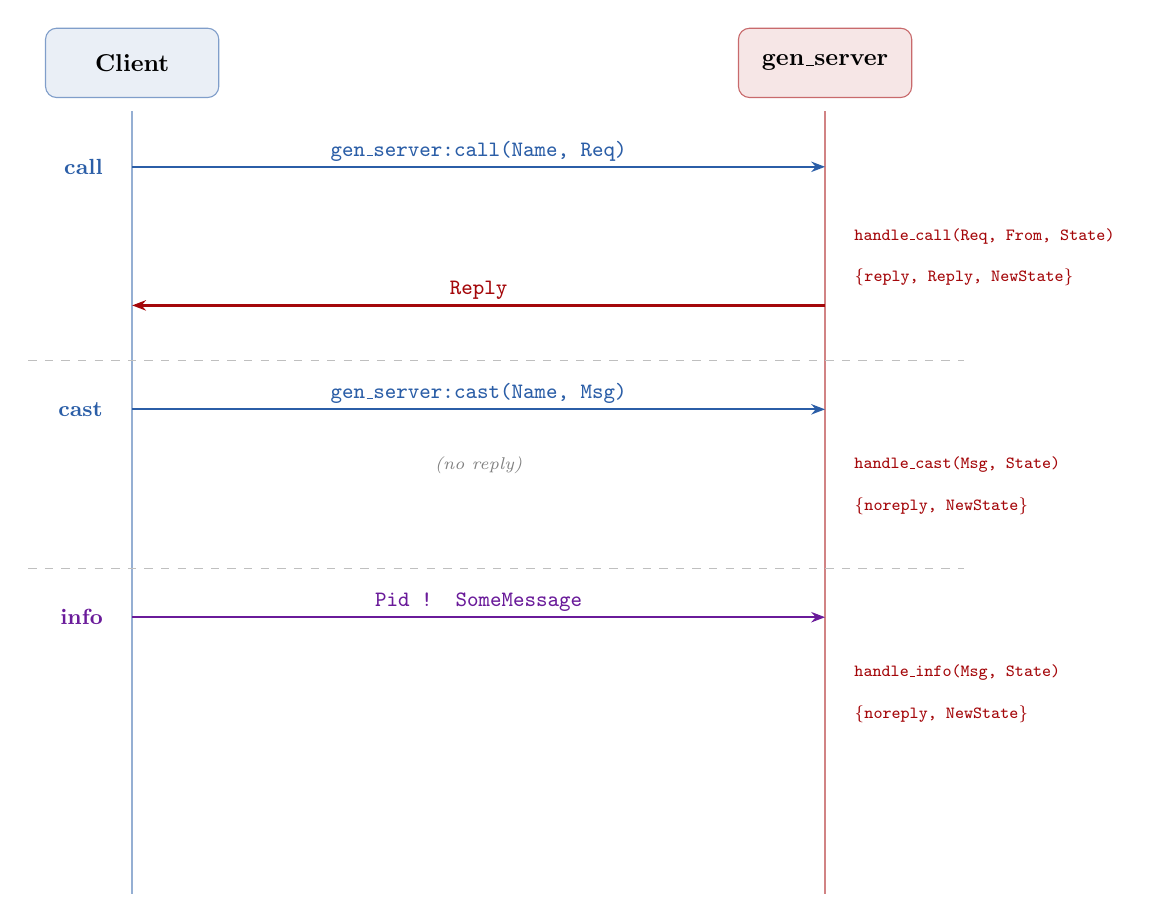
\begin{tikzpicture}[scale=0.88, every node/.style={scale=0.88},
    node distance=1cm,
    actor/.style={draw, rounded corners=4pt, fill=#1!10, draw=#1!60,
                  minimum width=2.5cm, minimum height=1cm, font=\bfseries},
    msg/.style={-{Stealth[length=5pt]}, thick, #1},
    lbl/.style={font=\small\ttfamily, fill=white, inner sep=2pt},
]
    % Actors
    \node[actor=erlblue] (client) at (0, 0) {Client};
    \node[actor=erlred] (server) at (10, 0) {gen\_server};

    % Timeline
    \draw[thick, erlblue!50] (0, -0.7) -- (0, -12);
    \draw[thick, erlred!50] (10, -0.7) -- (10, -12);

    % === call ===
    \node[font=\small\bfseries\color{erlblue}, anchor=east] at (-0.3, -1.5) {call};
    \draw[msg=erlblue] (0, -1.5) -- node[lbl, above] {gen\_server:call(Name, Req)} (10, -1.5);
    \node[font=\scriptsize\ttfamily, anchor=west, text=erlred] at (10.3, -2.5) {handle\_call(Req, From, State)};
    \node[font=\scriptsize\ttfamily, anchor=west, text=erlred] at (10.3, -3.1) {\{reply, Reply, NewState\}};
    \draw[msg=erlred] (10, -3.5) -- node[lbl, above] {Reply} (0, -3.5);

    % === cast ===
    \node[font=\small\bfseries\color{erlblue}, anchor=east] at (-0.3, -5) {cast};
    \draw[msg=erlblue] (0, -5) -- node[lbl, above] {gen\_server:cast(Name, Msg)} (10, -5);
    \node[font=\scriptsize\ttfamily, anchor=west, text=erlred] at (10.3, -5.8) {handle\_cast(Msg, State)};
    \node[font=\scriptsize\ttfamily, anchor=west, text=erlred] at (10.3, -6.4) {\{noreply, NewState\}};
    \node[font=\scriptsize\itshape\color{gray}] at (5, -5.8) {(no reply)};

    % === info ===
    \node[font=\small\bfseries\color{erlpurple}, anchor=east] at (-0.3, -8) {info};
    \draw[msg=erlpurple] (0, -8) -- node[lbl, above] {Pid ! SomeMessage} (10, -8);
    \node[font=\scriptsize\ttfamily, anchor=west, text=erlred] at (10.3, -8.8) {handle\_info(Msg, State)};
    \node[font=\scriptsize\ttfamily, anchor=west, text=erlred] at (10.3, -9.4) {\{noreply, NewState\}};

    % Dashed separators
    \draw[dashed, gray!50] (-1.5, -4.3) -- (12, -4.3);
    \draw[dashed, gray!50] (-1.5, -7.3) -- (12, -7.3);
\end{tikzpicture}
\caption{gen\_server 三种消息类型的流转过程}
\label{fig:message-flow}
\end{figure}


% ============================================================
% Section 5: Callback Functions
% ============================================================
\section{gen\_server 回调函数详解}

\subsection{init/1}

\begin{lstlisting}[style=erlangstyle, caption={init/1 返回值}]
init(Args) ->
    {ok, State}              %% Normal start
  | {ok, State, Timeout}     %% Start with timeout
  | {ok, State, hibernate}   %% Start and hibernate (save memory)
  | {stop, Reason}           %% Start failed
  | ignore                   %% Ignore start
\end{lstlisting}

示例：
\begin{lstlisting}[style=erlangstyle]
init(_Args) ->
    Frequencies = {get_frequencies(), []},
    {ok, Frequencies}.
\end{lstlisting}

\subsection{handle\_call/3}

处理 \texttt{gen\_server:call/2,3} 发来的同步请求。

\begin{lstlisting}[style=erlangstyle, caption={handle\_call/3 返回值}]
handle_call(Request, From, State) ->
    {reply, Reply, NewState}              %% Reply and continue
  | {reply, Reply, NewState, Timeout}     %% Reply, set timeout
  | {reply, Reply, NewState, hibernate}   %% Reply, hibernate
  | {noreply, NewState}                   %% No reply (manual reply)
  | {noreply, NewState, Timeout}          %% No reply, set timeout
  | {stop, Reason, Reply, NewState}       %% Reply then stop
  | {stop, Reason, NewState}              %% Stop (no reply)
\end{lstlisting}

\texttt{From} 参数是 \texttt{\{Pid, Tag\}} 元组，可用于 \texttt{gen\_server:reply/2}。

\subsection{handle\_cast/2}

处理 \texttt{gen\_server:cast/2} 发来的异步请求。

\begin{lstlisting}[style=erlangstyle, caption={handle\_cast/2 返回值}]
handle_cast(Msg, State) ->
    {noreply, NewState}              %% Continue
  | {noreply, NewState, Timeout}     %% Continue, set timeout
  | {noreply, NewState, hibernate}   %% Continue, hibernate
  | {stop, Reason, NewState}         %% Stop
\end{lstlisting}

\subsection{handle\_info/2}

处理所有非 call/cast 的消息（如 \texttt{Pid ! Msg}、系统消息等）。

\begin{lstlisting}[style=erlangstyle, caption={handle\_info/2 返回值}]
handle_info(Info, State) ->
    {noreply, NewState}              %% Continue
  | {noreply, NewState, Timeout}     %% Continue, set timeout
  | {stop, Reason, NewState}         %% Stop
\end{lstlisting}

常见的 Info 消息：
\begin{itemize}[leftmargin=2em]
    \item \texttt{timeout} --- 超时触发
    \item \texttt{\{'EXIT', Pid, Reason\}} --- 链接进程退出
    \item \texttt{\{'DOWN', Ref, process, Pid, Reason\}} --- 监视的进程退出
    \item 任何用 \texttt{!} 发送的普通消息
\end{itemize}

\subsection{terminate/2}

服务器即将终止时调用。

\begin{lstlisting}[style=erlangstyle]
terminate(Reason, State) ->
    ok.  %% Return value is ignored
\end{lstlisting}

\begin{warnbox}[注意]
只有在以下情况下 \texttt{terminate/2} 才会被调用：
\begin{itemize}
    \item 回调函数返回 \texttt{\{stop, ...\}}
    \item 进程收到 EXIT 信号且设置了 \texttt{process\_flag(trap\_exit, true)}
\end{itemize}
\end{warnbox}

\subsection{code\_change/3}

热代码升级时调用。

\begin{lstlisting}[style=erlangstyle]
code_change(OldVsn, State, Extra) ->
    {ok, NewState}.
\end{lstlisting}

\subsection{format\_status/2 (可选)}

自定义 \texttt{sys:get\_status/1} 的输出，可用于隐藏敏感信息。

\begin{lstlisting}[style=erlangstyle]
format_status(_Opt, [_ProcDict, {Available, Allocated}]) ->
    {data, [{"State", {{available, Available},
                       {allocated, Allocated}}}]}.
\end{lstlisting}

\subsection{回调函数全景图}

\begin{figure}[H]
\centering
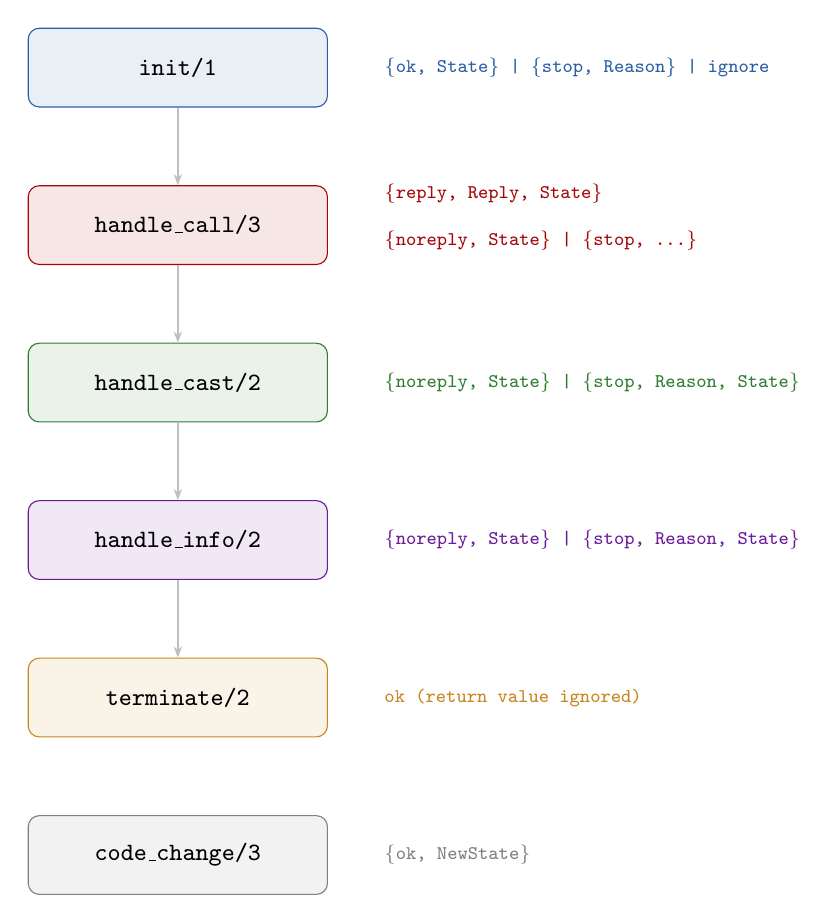
\begin{tikzpicture}[
    cb/.style={draw=#1, fill=#1!10, rounded corners=4pt,
               minimum width=3.8cm, minimum height=1cm, font=\small\bfseries\ttfamily},
    ret/.style={font=\scriptsize\ttfamily, text=#1, anchor=west},
]
    % Callbacks
    \node[cb=erlblue] (init) at (0, 0) {init/1};
    \node[cb=erlred] (hcall) at (0, -2) {handle\_call/3};
    \node[cb=erlgreen] (hcast) at (0, -4) {handle\_cast/2};
    \node[cb=erlpurple] (hinfo) at (0, -6) {handle\_info/2};
    \node[cb=erlyellow!80!black] (term) at (0, -8) {terminate/2};
    \node[cb=gray] (code) at (0, -10) {code\_change/3};

    % Return values
    \node[ret=erlblue] at (2.5, 0) {\{ok, State\} | \{stop, Reason\} | ignore};
    \node[ret=erlred] at (2.5, -1.6) {\{reply, Reply, State\}};
    \node[ret=erlred] at (2.5, -2.2) {\{noreply, State\} | \{stop, ...\}};
    \node[ret=erlgreen] at (2.5, -4) {\{noreply, State\} | \{stop, Reason, State\}};
    \node[ret=erlpurple] at (2.5, -6) {\{noreply, State\} | \{stop, Reason, State\}};
    \node[ret=erlyellow!80!black] at (2.5, -8) {ok (return value ignored)};
    \node[ret=gray] at (2.5, -10) {\{ok, NewState\}};

    % Flow arrows
    \draw[-{Stealth[length=4pt]}, thick, gray!50]
        (init.south) -- (hcall.north);
    \draw[-{Stealth[length=4pt]}, thick, gray!50]
        (hcall.south) -- (hcast.north);
    \draw[-{Stealth[length=4pt]}, thick, gray!50]
        (hcast.south) -- (hinfo.north);
    \draw[-{Stealth[length=4pt]}, thick, gray!50]
        (hinfo.south) -- (term.north);
\end{tikzpicture}
\caption{gen\_server 回调函数及其返回值}
\label{fig:callbacks}
\end{figure}


% ============================================================
% Section 6: Advanced Usage
% ============================================================
\section{进阶用法}

\subsection{显式回复 (gen\_server:reply/2)}

\begin{notebox}[源码文件]
\texttt{src/frequency\_reply.erl}
\end{notebox}

通常 \texttt{handle\_call} 通过 \texttt{\{reply, Reply, NewState\}} 回复客户端。但有时你需要：
\begin{itemize}[leftmargin=2em]
    \item 先回复客户端，再做耗时操作
    \item 在不同的进程中回复
    \item 条件性回复
\end{itemize}

\begin{lstlisting}[style=erlangstyle, caption={显式回复示例}]
handle_call({allocate, Pid}, From, Frequencies) ->
    {NewFrequencies, Reply} = allocate(Frequencies, Pid),
    %% Explicitly reply - client unblocks immediately
    gen_server:reply(From, Reply),
    %% Do post-reply work (client already got the response)
    io:format("Post-reply work: From=~p~n", [From]),
    %% Return noreply since we already replied
    {noreply, NewFrequencies}.
\end{lstlisting}

\begin{figure}[H]
\centering
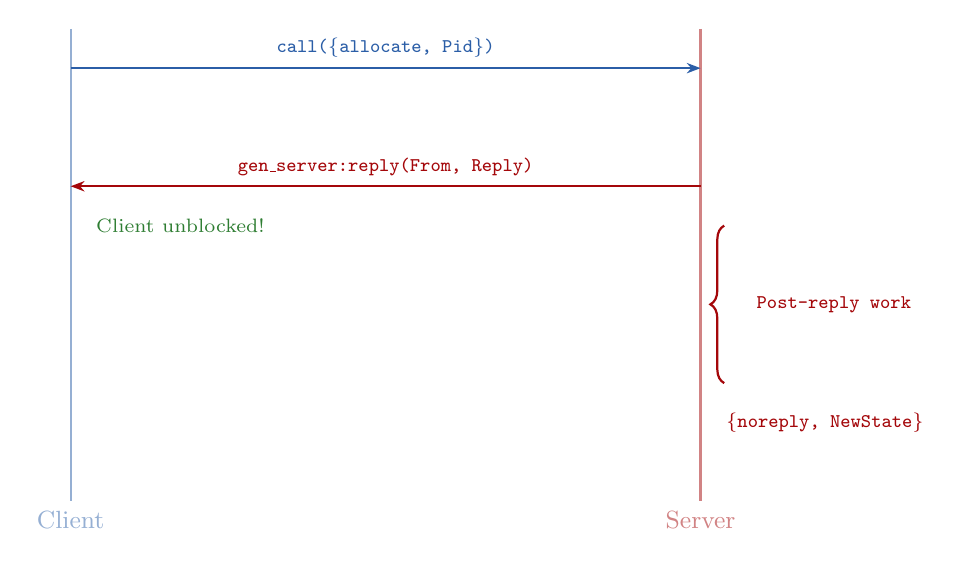
\begin{tikzpicture}[
    node distance=0.8cm,
]
    % Timeline
    \draw[thick, erlblue!50] (0, 0) -- (0, -6) node[below, font=\small] {Client};
    \draw[thick, erlred!50] (8, 0) -- (8, -6) node[below, font=\small] {Server};

    % Step 1: call
    \draw[-{Stealth[length=5pt]}, thick, erlblue]
        (0, -0.5) -- node[above, font=\scriptsize\ttfamily] {call(\{allocate, Pid\})} (8, -0.5);

    % Step 2: explicit reply
    \draw[-{Stealth[length=5pt]}, thick, erlred]
        (8, -2) -- node[above, font=\scriptsize\ttfamily] {gen\_server:reply(From, Reply)} (0, -2);

    % Client unblocked
    \node[font=\scriptsize\color{erlgreen}, anchor=west] at (0.2, -2.5) {Client unblocked!};

    % Step 3: post-reply work
    \draw[thick, erlred, decorate, decoration={brace, amplitude=5pt, mirror}]
        (8.3, -2.5) -- (8.3, -4.5) node[midway, right=8pt, font=\scriptsize\ttfamily] {Post-reply work};

    % Step 4: noreply
    \node[font=\scriptsize\ttfamily\color{erlred}, anchor=west] at (8.2, -5) {\{noreply, NewState\}};
\end{tikzpicture}
\caption{显式回复的时序图}
\label{fig:explicit-reply}
\end{figure}

\subsection{超时机制 (Timeout)}

\begin{notebox}[源码文件]
\texttt{src/timeout\_demo.erl}
\end{notebox}

gen\_server 支持在 init 和各个 handle\_* 回调中设置超时：

\begin{lstlisting}[style=erlangstyle, caption={超时机制示例}]
%% Set timeout in init
init(Timeout) ->
    {ok, #{timeout => Timeout, count => 0}, Timeout}.
%%                                          ^^^^^^^^
%%                                          Timeout in ms

%% Timeout triggers handle_info
handle_info(timeout, #{timeout := Timeout, count := Count} = State) ->
    io:format("Timeout #~p fired!~n", [Count + 1]),
    {noreply, State#{count := Count + 1}, Timeout}.
%%                                        ^^^^^^^^
%%                                        Reset timeout
\end{lstlisting}

\begin{warnbox}[重要]
每次收到\textbf{任何}消息都会重置超时计时器！
\end{warnbox}

\begin{figure}[H]
\centering
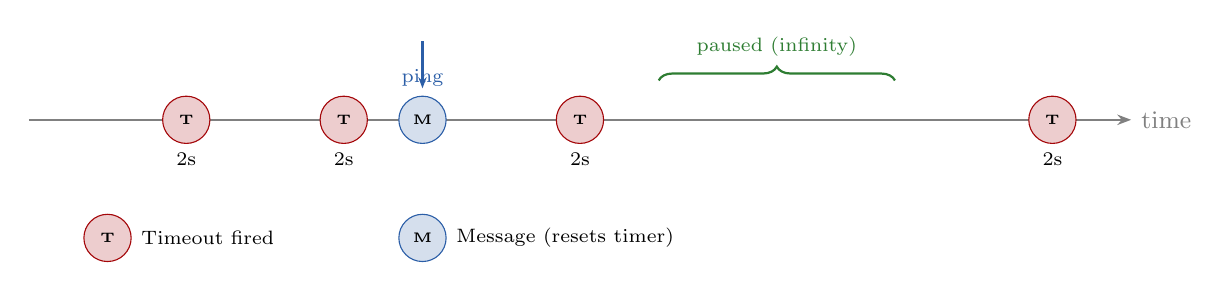
\begin{tikzpicture}[
    event/.style={circle, draw=#1, fill=#1!20, minimum size=6mm, font=\tiny\bfseries},
]
    % Timeline
    \draw[-{Stealth[length=5pt]}, thick, gray] (0, 0) -- (14, 0) node[right, font=\small] {time};

    % Timeout events
    \node[event=erlred] (t1) at (2, 0) {T};
    \node[event=erlred] (t2) at (4, 0) {T};

    % Message arrives - resets timer
    \node[event=erlblue] (m1) at (5, 0) {M};
    \node[font=\scriptsize\color{erlblue}, above=3mm] at (m1) {ping};
    \draw[-{Stealth[length=4pt]}, erlblue, thick] (5, 1) -- (5, 0.4);

    % More timeouts
    \node[event=erlred] (t3) at (7, 0) {T};

    % Pause
    \draw[thick, erlgreen, decorate, decoration={brace, amplitude=5pt}]
        (8, 0.5) -- (11, 0.5) node[midway, above=5pt, font=\scriptsize] {paused (infinity)};

    % Resume
    \node[event=erlred] (t4) at (13, 0) {T};

    % Labels
    \node[font=\scriptsize, below=3mm] at (t1) {2s};
    \node[font=\scriptsize, below=3mm] at (t2) {2s};
    \node[font=\scriptsize, below=3mm] at (t3) {2s};
    \node[font=\scriptsize, below=3mm] at (t4) {2s};

    % Legend
    \node[event=erlred, label=right:{\scriptsize Timeout fired}] at (1, -1.5) {T};
    \node[event=erlblue, label=right:{\scriptsize Message (resets timer)}] at (5, -1.5) {M};
\end{tikzpicture}
\caption{超时机制时间线}
\label{fig:timeout-timeline}
\end{figure}

\subsection{Call 超时与 start\_link vs start}

\begin{notebox}[源码文件]
\texttt{src/call\_timeout\_demo.erl}
\end{notebox}

\subsubsection{gen\_server:call 的超时}

\begin{lstlisting}[style=erlangstyle, caption={call 超时设置}]
%% Default 5-second timeout
gen_server:call(Server, Request).

%% Custom timeout
gen_server:call(Server, Request, Timeout).

%% Never timeout
gen_server:call(Server, Request, infinity).
\end{lstlisting}

\begin{warnbox}[关键点]
超时时，\textbf{客户端崩溃}，但\textbf{服务器继续运行}！
\end{warnbox}

\subsubsection{start\_link vs start}

\begin{table}[H]
\centering
\begin{tabular}{@{}lccc@{}}
\toprule
 & \textbf{start\_link} & \textbf{start} \\
\midrule
链接           & $\checkmark$ & --- \\
调用者崩溃     & 服务器也崩溃 & 服务器不受影响 \\
服务器崩溃     & 调用者收到 EXIT & 调用者不受影响 \\
用途           & 生产环境 (配合 supervisor) & 开发测试 \\
\bottomrule
\end{tabular}
\caption{start\_link vs start 对比}
\label{tab:start-link-vs-start}
\end{table}

\begin{figure}[H]
\centering
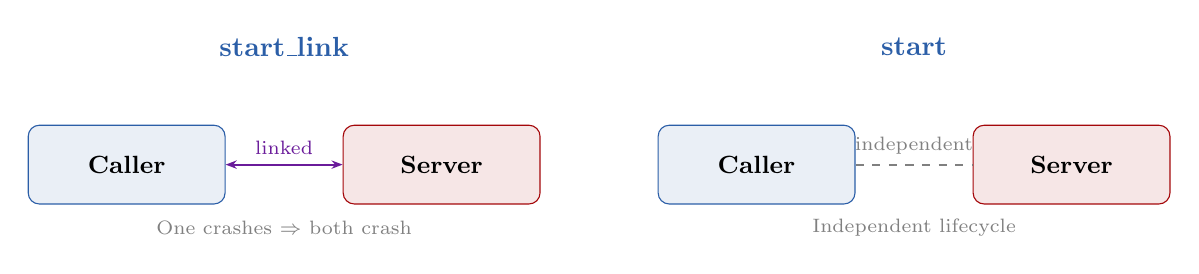
\begin{tikzpicture}[
    proc/.style={draw=#1, fill=#1!10, rounded corners=4pt,
                 minimum width=2.5cm, minimum height=1cm, font=\small\bfseries},
]
    % start_link scenario
    \node[font=\bfseries\color{erlblue}] at (0, 2) {start\_link};
    \node[proc=erlblue] (caller1) at (-2, 0.5) {Caller};
    \node[proc=erlred] (server1) at (2, 0.5) {Server};
    \draw[thick, erlpurple, {Stealth[length=4pt]}-{Stealth[length=4pt]}]
        (caller1) -- node[above, font=\scriptsize] {linked} (server1);
    \node[font=\scriptsize\color{gray}] at (0, -0.3) {One crashes $\Rightarrow$ both crash};

    % start scenario
    \node[font=\bfseries\color{erlblue}] at (8, 2) {start};
    \node[proc=erlblue] (caller2) at (6, 0.5) {Caller};
    \node[proc=erlred] (server2) at (10, 0.5) {Server};
    \draw[thick, gray, dashed]
        (caller2) -- node[above, font=\scriptsize] {independent} (server2);
    \node[font=\scriptsize\color{gray}] at (8, -0.3) {Independent lifecycle};
\end{tikzpicture}
\caption{start\_link vs start 进程关系}
\label{fig:start-link-vs-start}
\end{figure}


% ============================================================
% Section 7: Process Registration
% ============================================================
\section{进程注册方式}

\begin{notebox}[源码文件]
\texttt{src/kv\_store.erl}
\end{notebox}

gen\_server 支持多种进程注册方式：

\subsection{本地注册 \{local, Name\}}

\begin{lstlisting}[style=erlangstyle]
gen_server:start_link({local, my_server}, ?MODULE, [], []).
%% Only visible on current node
%% Call by name: gen_server:call(my_server, Request)
\end{lstlisting}

\subsection{全局注册 \{global, Name\}}

\begin{lstlisting}[style=erlangstyle]
gen_server:start_link({global, my_server}, ?MODULE, [], []).
%% Visible on all connected nodes
%% Call: gen_server:call({global, my_server}, Request)
\end{lstlisting}

\subsection{不注册（使用 PID）}

\begin{lstlisting}[style=erlangstyle]
{ok, Pid} = gen_server:start_link(?MODULE, [], []).
%% Call by PID only: gen_server:call(Pid, Request)
%% Can start multiple instances!
\end{lstlisting}

\subsection{远程节点调用 \{Name, Node\}}

\begin{lstlisting}[style=erlangstyle]
%% Call a locally registered process on a remote node
gen_server:call({my_server, 'node1@hostname'}, Request).
\end{lstlisting}

\subsection{server\_ref 完整类型}

\begin{figure}[H]
\centering
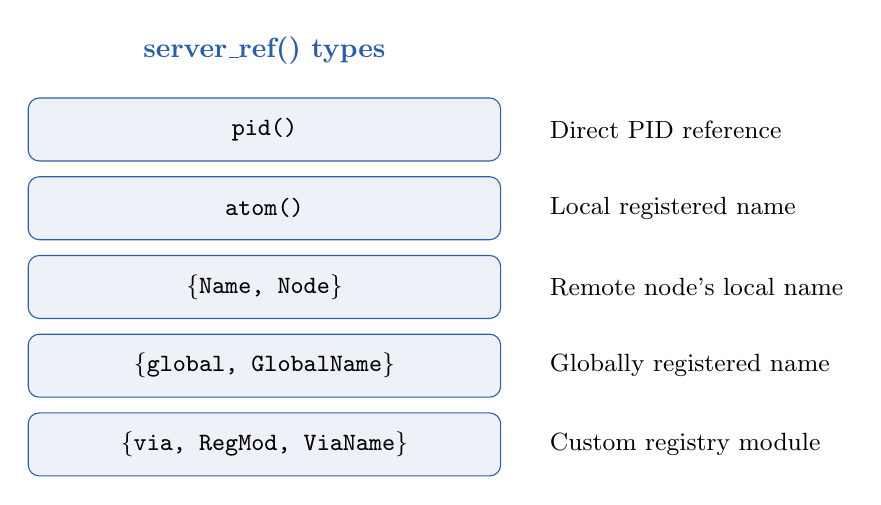
\begin{tikzpicture}[
    ref/.style={draw=erlblue, fill=erlblue!8, rounded corners=4pt,
                minimum width=6cm, minimum height=0.8cm, font=\small\ttfamily},
    desc/.style={font=\small, anchor=west},
]
    \node[font=\bfseries\color{erlblue}] at (0, 3.5) {server\_ref() types};

    \node[ref] (r1) at (0, 2.5) {pid()};
    \node[ref] (r2) at (0, 1.5) {atom()};
    \node[ref] (r3) at (0, 0.5) {\{Name, Node\}};
    \node[ref] (r4) at (0, -0.5) {\{global, GlobalName\}};
    \node[ref] (r5) at (0, -1.5) {\{via, RegMod, ViaName\}};

    \node[desc] at (3.5, 2.5) {Direct PID reference};
    \node[desc] at (3.5, 1.5) {Local registered name};
    \node[desc] at (3.5, 0.5) {Remote node's local name};
    \node[desc] at (3.5, -0.5) {Globally registered name};
    \node[desc] at (3.5, -1.5) {Custom registry module};
\end{tikzpicture}
\caption{server\_ref() 类型一览}
\label{fig:server-ref}
\end{figure}


% ============================================================
% Section 8: Distributed Communication
% ============================================================
\section{分布式节点通信}

\begin{notebox}[源码文件]
\texttt{src/distributed\_demo.erl}
\end{notebox}

\subsection{本地 PID vs 远程 PID}

这是理解分布式 Erlang 的关键：

\begin{figure}[H]
\centering
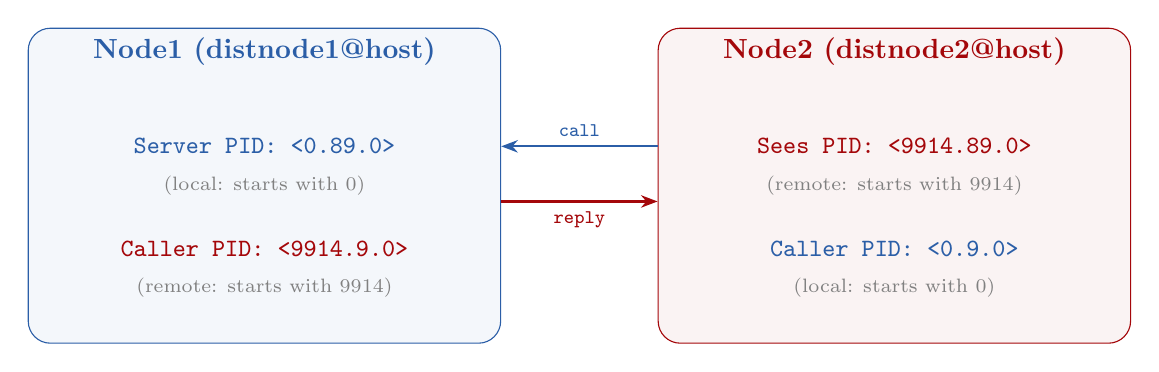
\begin{tikzpicture}[
    node box/.style={draw=#1, fill=#1!5, rounded corners=8pt,
                     minimum width=6cm, minimum height=4cm},
    pid/.style={font=\ttfamily\small, text=#1},
]
    % Node 1
    \node[node box=erlblue] (n1) at (0, 0) {};
    \node[font=\bfseries\color{erlblue}, anchor=north] at (n1.north) {Node1 (distnode1@host)};
    \node[pid=erlblue] at (0, 0.5) {Server PID: \textbf{<0.89.0>}};
    \node[font=\scriptsize\color{gray}] at (0, 0) {(local: starts with 0)};
    \node[pid=erlred] at (0, -0.8) {Caller PID: <9914.9.0>};
    \node[font=\scriptsize\color{gray}] at (0, -1.3) {(remote: starts with 9914)};

    % Node 2
    \node[node box=erlred] (n2) at (8, 0) {};
    \node[font=\bfseries\color{erlred}, anchor=north] at (n2.north) {Node2 (distnode2@host)};
    \node[pid=erlred] at (8, 0.5) {Sees PID: \textbf{<9914.89.0>}};
    \node[font=\scriptsize\color{gray}] at (8, 0) {(remote: starts with 9914)};
    \node[pid=erlblue] at (8, -0.8) {Caller PID: <0.9.0>};
    \node[font=\scriptsize\color{gray}] at (8, -1.3) {(local: starts with 0)};

    % Arrows
    \draw[-{Stealth[length=6pt]}, thick, erlblue]
        ([yshift=5mm]n2.west) -- node[above, font=\scriptsize\ttfamily] {call} ([yshift=5mm]n1.east);
    \draw[-{Stealth[length=6pt]}, thick, erlred]
        ([yshift=-2mm]n1.east) -- node[below, font=\scriptsize\ttfamily] {reply} ([yshift=-2mm]n2.west);
\end{tikzpicture}
\caption{本地 PID vs 远程 PID --- 同一个进程在不同节点上的 PID 表示不同}
\label{fig:pid-difference}
\end{figure}

\subsection{实际演示}

\textbf{Terminal 1 (node1)：启动服务器}
\begin{lstlisting}[style=shellstyle]
$ erl -sname node1 -setcookie demo
(node1@HOST)1> distributed_demo:start_link().
[distributed_demo] Started on node='node1@HOST', PID=<0.89.0>
{ok,<0.89.0>}
(node1@HOST)2> distributed_demo:store(greeting, hello_from_node1).
ok
\end{lstlisting}

\textbf{Terminal 2 (node2)：连接并远程调用}
\begin{lstlisting}[style=shellstyle]
$ erl -sname node2 -setcookie demo
(node2@HOST)1> net_adm:ping('node1@HOST').
pong
(node2@HOST)2> distributed_demo:remote_get_info('node1@HOST').
\end{lstlisting}

\subsection{全局注册的分布式场景}

\begin{lstlisting}[style=shellstyle]
# Terminal 1
$ erl -sname apple -setcookie test
(apple@host)1> kv_store:start_link_global().
{ok,<0.89.0>}

# Terminal 2
$ erl -sname pear -setcookie test
(pear@host)1> net_adm:ping('apple@host').
pong
(pear@host)2> global:whereis_name(kv_store_global).
<9435.89.0>                    %% Remote PID!
(pear@host)3> kv_store:put_global(key1, value1).
ok

# Start again will fail (globally unique)
(pear@host)5> kv_store:start_link_global().
{error,{already_started,<9435.89.0>}}
\end{lstlisting}


% ============================================================
% Section 9: Best Practices
% ============================================================
\section{最佳实践与常见陷阱}

\subsection{最佳实践}

\begin{enumerate}[leftmargin=2em]
    \item \textbf{始终使用 start\_link}：在生产环境中，gen\_server 应该始终通过 supervisor 启动，使用 \texttt{start\_link}。

    \item \textbf{保持 handle\_call 快速}：默认 5 秒超时，长时间操作应该用 cast 或 spawn 子进程。

    \item \textbf{合理使用 call vs cast}：
    \begin{itemize}
        \item \texttt{call}：需要返回值、需要确认操作完成
        \item \texttt{cast}：不需要返回值、fire-and-forget
    \end{itemize}

    \item \textbf{handle\_info 处理未知消息}：总是添加一个 catch-all 子句。

    \item \textbf{terminate 中做清理}：释放资源、关闭连接等。

    \item \textbf{使用 format\_status 隐藏敏感信息}：密码、token 等不应出现在崩溃日志中。
\end{enumerate}

\subsection{常见陷阱}

\subsubsection{陷阱 1：在 shell 中使用 start\_link}

\begin{lstlisting}[style=erlangstyle, caption={Shell 中 start\_link 的陷阱}]
%% Shell process and gen_server are linked
%% If gen_server crashes, shell also crashes (then restarts)
1> gen_server:start_link({local, my}, my_mod, [], []).
{ok,<0.83.0>}
2> gen_server:call(my, crash).
** exception exit: ...
3> self().
<0.88.0>   %% Shell process has changed!
\end{lstlisting}

\subsubsection{陷阱 2：call 超时后的残留消息}

\begin{lstlisting}[style=erlangstyle, caption={超时后的残留消息问题}]
%% After client timeout, server's reply still arrives
%% This reply stays in client's message queue
try
    gen_server:call(Server, Request, 1000)
catch
    exit:{timeout, _} ->
        %% Server may reply later, message stays in queue
        %% Need to flush or use alias (OTP 24+)
        ok
end.
\end{lstlisting}

\subsubsection{陷阱 3：在 handle\_call 中调用自己}

\begin{lstlisting}[style=erlangstyle, caption={死锁！不要在 handle\_call 中调用自己}]
%% DEADLOCK! gen_server is single-process,
%% cannot call itself while handling a message
handle_call(request1, _From, State) ->
    Result = gen_server:call(self(), request2),  %% DEADLOCK!
    {reply, Result, State}.
\end{lstlisting}

\begin{figure}[H]
\centering
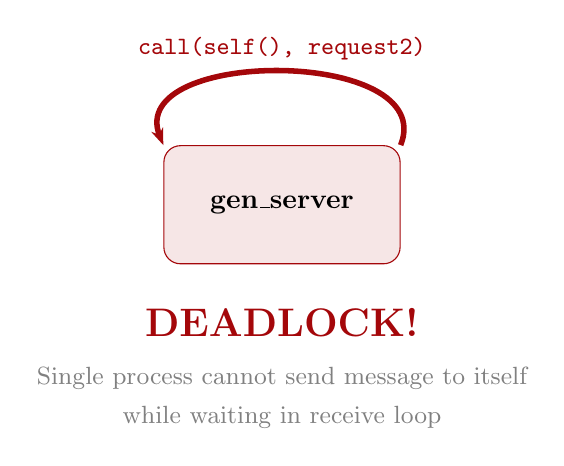
\begin{tikzpicture}
    \node[draw=erlred, fill=erlred!10, rounded corners=6pt,
          minimum width=3cm, minimum height=1.5cm, font=\bfseries] (gs) at (0,0) {gen\_server};

    \draw[-{Stealth[length=6pt]}, thick, erlred, line width=2pt]
        (gs.north east) .. controls (2, 2) and (-2, 2) .. (gs.north west)
        node[midway, above, font=\small\ttfamily] {call(self(), request2)};

    \node[font=\Large\bfseries\color{erlred}] at (0, -1.5) {DEADLOCK!};
    \node[font=\small\color{gray}] at (0, -2.2) {Single process cannot send message to itself};
    \node[font=\small\color{gray}] at (0, -2.7) {while waiting in receive loop};
\end{tikzpicture}
\caption{死锁：gen\_server 调用自己}
\label{fig:deadlock}
\end{figure}

\subsection{调试工具}

\begin{lstlisting}[style=erlangstyle, caption={gen\_server 调试工具}]
%% Get server status
sys:get_status(ServerRef).

%% Trace messages
sys:trace(ServerRef, true).

%% Get statistics
sys:statistics(ServerRef, true).
sys:statistics(ServerRef, get).

%% Suspend / Resume
sys:suspend(ServerRef).
sys:resume(ServerRef).
\end{lstlisting}


% ============================================================
% Section 10: Quick Reference
% ============================================================
\section{快速参考}

\subsection{启动函数}

\begin{table}[H]
\centering
\small
\begin{tabular}{@{}lcc@{}}
\toprule
\textbf{函数} & \textbf{链接} & \textbf{说明} \\
\midrule
\texttt{start\_link(\{local,N\}, Mod, Args, Opts)} & $\checkmark$ & 本地注册+链接 \\
\texttt{start\_link(\{global,N\}, Mod, Args, Opts)} & $\checkmark$ & 全局注册+链接 \\
\texttt{start\_link(Mod, Args, Opts)} & $\checkmark$ & 不注册+链接 \\
\texttt{start(\{local,N\}, Mod, Args, Opts)} & --- & 本地注册 \\
\texttt{start(\{global,N\}, Mod, Args, Opts)} & --- & 全局注册 \\
\bottomrule
\end{tabular}
\caption{gen\_server 启动函数}
\end{table}

\subsection{客户端函数}

\begin{table}[H]
\centering
\small
\begin{tabular}{@{}llp{5.5cm}@{}}
\toprule
\textbf{函数} & \textbf{类型} & \textbf{说明} \\
\midrule
\texttt{call(Ref, Request)} & 同步 & 默认5秒超时 \\
\texttt{call(Ref, Request, Timeout)} & 同步 & 自定义超时 \\
\texttt{cast(Ref, Msg)} & 异步 & 无返回值 \\
\texttt{reply(From, Reply)} & --- & 显式回复 \\
\texttt{stop(Ref)} & 同步 & 停止服务器 \\
\texttt{multi\_call(Nodes, Name, Req)} & 同步 & 多节点调用 \\
\texttt{abcast(Nodes, Name, Msg)} & 异步 & 多节点广播 \\
\bottomrule
\end{tabular}
\caption{gen\_server 客户端函数}
\end{table}

\subsection{回调函数返回值速查}

\begin{figure}[H]
\centering
\begin{tcolorbox}[colback=codebg, colframe=codeborder, arc=2mm, boxrule=0.5pt,
                  title={\textbf{Callback Return Values Quick Reference}},
                  fonttitle=\bfseries\ttfamily, width=\textwidth]
\small\ttfamily
\textbf{init/1:} \\
\quad \{ok, State\} | \{ok, State, Timeout\} | \{stop, Reason\} | ignore \\[6pt]
\textbf{handle\_call/3:} \\
\quad \{reply, Reply, State\} \\
\quad \{reply, Reply, State, Timeout\} \\
\quad \{noreply, State\} \\
\quad \{noreply, State, Timeout\} \\
\quad \{stop, Reason, Reply, State\} \\
\quad \{stop, Reason, State\} \\[6pt]
\textbf{handle\_cast/2:} \\
\quad \{noreply, State\} \\
\quad \{noreply, State, Timeout\} \\
\quad \{stop, Reason, State\} \\[6pt]
\textbf{handle\_info/2:} \\
\quad \{noreply, State\} \\
\quad \{noreply, State, Timeout\} \\
\quad \{stop, Reason, State\} \\[6pt]
\textbf{terminate/2:} \\
\quad ok \quad (return value is ignored) \\[6pt]
\textbf{code\_change/3:} \\
\quad \{ok, NewState\}
\end{tcolorbox}
\end{figure}

\subsection{源码文件列表}

\begin{table}[H]
\centering
\small
\begin{tabular}{@{}ll@{}}
\toprule
\textbf{文件} & \textbf{说明} \\
\midrule
\texttt{src/frequency\_raw.erl} & Step 1: 纯 Erlang 进程实现 \\
\texttt{src/my\_server.erl} & Step 2: 自定义通用服务器 \\
\texttt{src/frequency\_generic.erl} & Step 2: 使用自定义通用服务器 \\
\texttt{src/frequency\_otp.erl} & Step 3: OTP gen\_server 实现 \\
\texttt{src/frequency\_reply.erl} & 显式回复 (gen\_server:reply) \\
\texttt{src/timeout\_demo.erl} & 超时机制演示 \\
\texttt{src/call\_timeout\_demo.erl} & Call 超时与 start vs start\_link \\
\texttt{src/kv\_store.erl} & 多种注册方式 (local/global/pid) \\
\texttt{src/distributed\_demo.erl} & 分布式节点通信 \\
\bottomrule
\end{tabular}
\caption{源码文件列表}
\end{table}

\subsection{Makefile 命令}

\begin{table}[H]
\centering
\small
\begin{tabular}{@{}ll@{}}
\toprule
\textbf{命令} & \textbf{说明} \\
\midrule
\texttt{make compile} & 编译所有文件 \\
\texttt{make run\_raw} & Step 1: 纯 Erlang 进程 \\
\texttt{make run\_generic} & Step 2: 自定义通用服务器 \\
\texttt{make run\_otp} & Step 3: OTP gen\_server \\
\texttt{make run\_reply} & 显式回复演示 \\
\texttt{make run\_timeout} & 超时演示 (约15秒) \\
\texttt{make run\_call\_timeout} & Call 超时演示 \\
\texttt{make run\_kv\_local} & KV Store 本地注册 \\
\texttt{make run\_kv\_unnamed} & KV Store 无名 (PID) \\
\texttt{make run\_distributed} & 分布式演示 \\
\texttt{make run\_all} & 运行所有演示 \\
\texttt{make clean} & 清理编译文件 \\
\bottomrule
\end{tabular}
\caption{Makefile 命令速查}
\end{table}

\end{document}
